\section{Results without hardware}\label{sec:simulation}

Two things can be checked before the campaign: the model form on the
lab's published tables, and the analysis of
§\ref{sec:prior}--\ref{sec:baselines} on a synthetic population whose
truth is known.

\subsection{Reanalysis of the lab's tables}\label{sec:lab-tables}

On the digital twin's public 7×7 tables (one value per cell, powers
60--120), the leave-one-cell-out error of the lab's cubic fit of \(v\)
is 0.53 cm/s, worse than a plane at 0.48 cm/s, and the coefficients
pasted into the inverse step are truncated (in-sample error 0.38 → 0.63
cm/s). The lab's own lookup tables reach only about 44 \% of the
targets in their \((v,\omega)\) box; the rest is silently projected.
The grey-box map fitted to the same 49 points is the only real-data
check of the model form available before the campaign. With the dead
zones constrained below the grid's lowest power, the linear variant's
leave-one-cell-out error is 0.50 cm/s in \(v\) and 0.23 rad/s in
\(\omega\), and the variant with the \(f_L f_R\) term reaches 0.47
cm/s; a plane gives 0.48 cm/s in \(v\) and the quadratic 0.215 rad/s in
\(\omega\). On 49 single measurements the grey-box form therefore
matches low-order polynomials in accuracy, and the dead zone it carries
is imposed by the bound rather than fitted: a grid that starts at power
60 does not identify \(p_0\) and \(\gamma\), which is why the
protocol's grid includes 0 and 55. What the form adds on these tables is
the closed-form inverse and a feasible region, which covers 38 \% of the
lookup table's box. The \texttt{cor} variant gives \(\bar d = 2.3\) mm
with a cell-bootstrap 95 \% interval of \(-0.1\) to 4.9 mm, so on 49
points the mean offset is not distinguishable from zero; the table's
\(v\) is a centre-of-mass speed magnitude, so this \(\bar d\) is that
point's offset, not a marker's.

\subsection{Simulation: synthetic population}

Robots are drawn around a reference map shaped like the twin's envelope
(4--12 cm/s, clockwise bias at \(L = R\)): per-robot dead zones (SD 2
drive units), exponents (SD 0.03), lognormal motor gains (SD 5 \%),
yaw-rate intercept (SD 0.05 rad/s) and speed intercepts (SD 1 mm/s),
with per-day lognormal gain drift (SD 2 \%) and dead-zone drift (SD 1
unit), and per-segment twist noise of 3 mm/s, 2 mm/s and 0.05 rad/s. At
this ``spread 1'' the between-robot SD on the grid is about 0.6 cm/s in
\(u_1\) and 0.30 rad/s in \(\omega\), the day SD a quarter to a third
of that; spreads 0.3 and 3 bracket it. Every robot's pool is the full
grid with five replicates (405 segments), scored against its noise-free
truth. All numbers that follow are synthetic. The population is drawn
from the model family that is then fitted, so the study can only show
that the estimators work when their assumptions hold; it has no battery
term, no high-drive reversal and no lag.

\subsection{Variance decomposition}

With eight robots, two days and five replicates the nested estimator
recovers the injected robot SDs of \(u_1\) and \(\omega\) within 4 \%
at all three spreads and the day SDs within 3 \%, except \(u_1\) at
the smallest spread, where a day component of 0.4 mm/s sits below the
3 mm/s segment noise and is overestimated by about 70 \%
(Table~\ref{tab:1} shows spread 1); \(u_2\) is at the noise floor in
this population and its robot component is poorly determined, as it
would be on real robots whose lateral slip is small.

\begin{table}[t]
\caption{Simulation, spread 1: estimated (true) standard deviations of the robot, day and segment components, and their fractions of the total variance.}
\label{tab:1}
\centering\scriptsize\setlength{\tabcolsep}{3pt}
\begin{tabular}{lcccc}
\toprule
output & robot & day & segment & r / d / s \\
\midrule
\(u_1\) {[}m/s{]} & 0.0060 (0.0060) & 0.0014 (0.0014) & 0.0030 (0.0030) & 0.76 / 0.04 / 0.19 \\
\(u_2\) {[}m/s{]} & 0.0010 (0.0010) & 0.0004 (0.0001) & 0.0020 (0.0020) & 0.20 / 0.03 / 0.77 \\
\(\omega\) {[}rad/s{]} & 0.300 (0.308) & 0.101 (0.101) & 0.050 (0.050) & 0.88 / 0.10 / 0.02 \\
\bottomrule
\end{tabular}
\end{table}


\subsection{Few-shot calibration}\label{sec:sim-fewshot}

Fig.~\ref{fig:sim-fewshot} and Table~\ref{tab:2} give the
leave-one-robot-out error against the number of segments \(k\): the
RMSE over the grid in score units, where one unit is the residual
scaling of §\ref{sec:forward-map} (0.5 cm/s in \(u_1\) and \(u_2\),
0.1 rad/s in \(\omega\)), as the median over eight held-out robots and
three random subsets. The full 405-segment fit scores 0.050; the prior
mean with no data about 2.0.

\begin{figure}[t]
\centering
% Few-shot error vs k on the synthetic population (spread 1): numbers from
% ../results/loro_spread1.txt (popsim.py loro), medians over 8 held-out robots x 3 subsets.
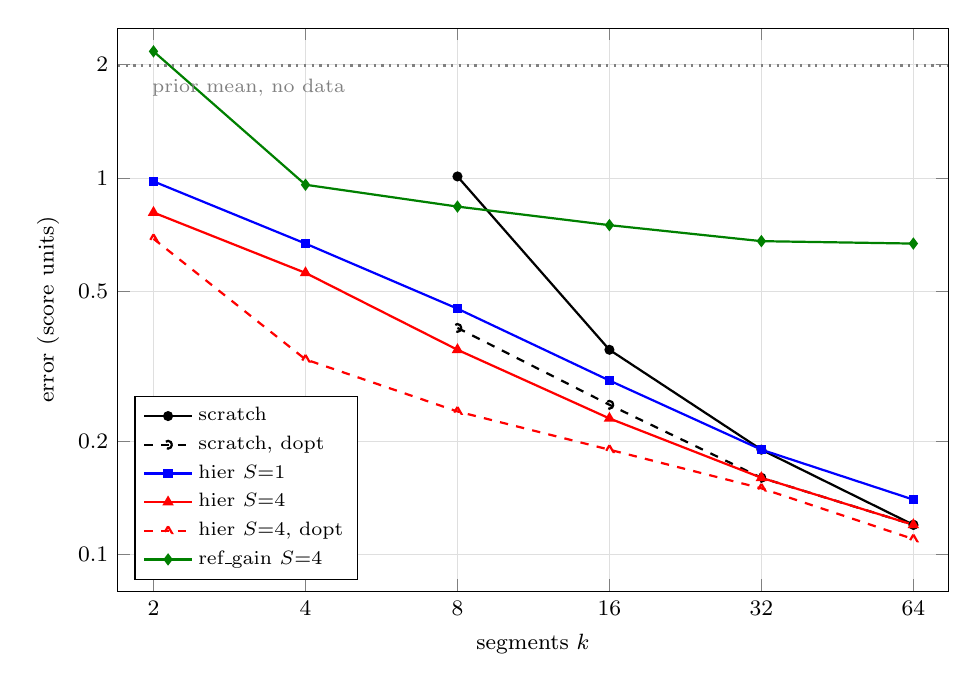
\begin{tikzpicture}
\begin{loglogaxis}[
  width=\columnwidth, height=0.72\columnwidth,
  xlabel={segments $k$}, ylabel={error (score units)},
  xtick={2,4,8,16,32,64}, xticklabels={2,4,8,16,32,64},
  ytick={0.1,0.2,0.5,1,2}, yticklabels={0.1,0.2,0.5,1,2},
  ymin=0.08, ymax=2.5, xmin=1.7, xmax=75,
  legend style={font=\scriptsize, at={(0.02,0.02)}, anchor=south west, cells={anchor=west}},
  grid=major, grid style={gray!25}, tick label style={font=\footnotesize}, label style={font=\footnotesize},
]
\addplot[black, thick, mark=*, mark size=1.4] coordinates {(8,1.01) (16,0.35) (32,0.19) (64,0.12)};
\addlegendentry{scratch}
\addplot[black, thick, dashed, mark=o, mark size=1.4] coordinates {(8,0.40) (16,0.25) (32,0.16) (64,0.12)};
\addlegendentry{scratch, dopt}
\addplot[blue, thick, mark=square*, mark size=1.3] coordinates {(2,0.98) (4,0.67) (8,0.45) (16,0.29) (32,0.19) (64,0.14)};
\addlegendentry{hier $S{=}1$}
\addplot[red, thick, mark=triangle*, mark size=1.6] coordinates {(2,0.81) (4,0.56) (8,0.35) (16,0.23) (32,0.16) (64,0.12)};
\addlegendentry{hier $S{=}4$}
\addplot[red, thick, dashed, mark=triangle, mark size=1.6] coordinates {(2,0.69) (4,0.33) (8,0.24) (16,0.19) (32,0.15) (64,0.11)};
\addlegendentry{hier $S{=}4$, dopt}
\addplot[green!50!black, thick, mark=diamond*, mark size=1.6] coordinates {(2,2.17) (4,0.96) (8,0.84) (16,0.75) (32,0.68) (64,0.67)};
\addlegendentry{ref\_gain $S{=}4$}
\addplot[gray, dotted, thick, domain=1.7:75] {0.05};
\addplot[gray, dotted, thick, domain=1.7:75] {1.99};
\node[gray, font=\scriptsize, anchor=south west] at (axis cs:1.9,0.052) {full grid};
\node[gray, font=\scriptsize, anchor=north west] at (axis cs:1.9,1.95) {prior mean, no data};
\end{loglogaxis}
\end{tikzpicture}

\caption{Simulation, spread 1: few-shot error against the number of segments \(k\) (median over held-out robots and subsets). Solid: random segments; dashed: D-optimal segments. The full-grid fit (405 segments) scores 0.05.}
\label{fig:sim-fewshot}
\end{figure}

\begin{table*}[t]
\caption{Simulation, spread 1: few-shot error (score units, median over held-out robots and subsets) against the number of segments \(k\). \texttt{scratch}: fit on the \(k\) segments alone; \texttt{hier} \(S\): MAP fit under a prior from \(S\) robots; \texttt{ref\_gain}: affine correction of the prior mean; \texttt{dopt}: D-optimal instead of random segments. ``--'': not fittable.}
\label{tab:2}
\centering\footnotesize
\begin{tabular}{lcccccccc}
\toprule
\(k\) & scratch & hier S=1 & hier S=2 & hier S=4 & ref\_gain S=4 & scratch, dopt & hier S=1, dopt & hier S=4, dopt \\
\midrule
2 & -- & 0.98 & 0.82 & 0.81 & 2.17 & -- & 0.91 & 0.69 \\
4 & -- & 0.67 & 0.56 & 0.56 & 0.96 & -- & 0.39 & 0.33 \\
8 & 1.01 & 0.45 & 0.35 & 0.35 & 0.84 & 0.40 & 0.31 & 0.24 \\
16 & 0.35 & 0.29 & 0.25 & 0.23 & 0.75 & 0.25 & 0.22 & 0.19 \\
32 & 0.19 & 0.19 & 0.17 & 0.16 & 0.68 & 0.16 & 0.16 & 0.15 \\
64 & 0.12 & 0.14 & 0.14 & 0.12 & 0.67 & 0.12 & 0.12 & 0.11 \\
\bottomrule
\end{tabular}
\end{table*}


In this synthetic population the prior pays below about 32 segments: at
\(k = 8\) the MAP fit with a four-robot prior scores 0.35 against 1.01
for fitting from scratch with random cells (2.9×) and 0.24 against 0.40
with designed ones (1.7×), and fitting from scratch is not possible
below \(k = 8\) at all; at \(k = 16\) the margin is 1.3--1.5 and by
\(k = 32\) it is gone. D-optimal cells roughly halve the segments needed
at small \(k\): eight designed segments with a four-robot prior match
sixteen random ones. The master/slave baseline plateaus at 0.6--0.9
because an affine correction of a reference map cannot absorb
differences in dead zone and exponent. Sixteen designed segments, about
two minutes of driving, leave an error of 0.19 score units, i.e. 0.95
mm/s and 0.019 rad/s, which is 16 \% of the between-robot spread in
\(u_1\) and 6 \% in \(\omega\), and below the 3 mm/s and 0.05 rad/s
noise of a single segment. A budget of ten minutes, about 75 segments at
the protocol's 8 s per segment, would therefore be generous if real
robots followed the model family; whether they do is what the full grids
of phase B test. The 95 \% intervals of the MAP fit cover the true mean
twist 84--95 \% of the time at \(k \ge 4\) (the floor heuristics are
slightly narrow) and 99--100 \% at \(k = 0\) (the prior is wide).

\subsection{How many calibrated
robots?}\label{sec:sim-power}

Repeating the study over eight simulated populations for fleets of
\(N = 4\), 6 and 8 fully calibrated robots and spreads 0.3, 1 and 3
(Table~\ref{tab:3}) separates the fleet size \(N\) from the prior size
\(S\). The fleet size sets how well the between-robot spread is
\emph{known}: the 10--90 \% band of the estimated robot SD of \(\omega\),
relative to the population value, spans roughly 0.6--1.1 at four robots
and 0.7--1.2 at eight. The expected narrowing of a standard deviation's
sampling error with \(N\), \(\approx 1/\sqrt{2(N-1)}\), is not resolved
by eight populations per cell, so the sweep says that four to eight
full grids leave the spread uncertain by roughly a quarter and no more
than that. The fleet size barely changes how well a \emph{new} robot is
calibrated: at \(k = 16\) a prior from \(S = N-1\) robots gives
0.20--0.29 at every spread except the largest with four robots (0.32),
and a one-robot prior 0.25--0.41; the larger prior lowers the \(k = 16\)
error by 0.02--0.09 in every row, while at \(k = 4\) it helps with six
or eight robots at the two larger spreads and not with four. If real
robots behaved like this population, five or six full grids would be a
reasonable phase B and more would buy a tighter spread estimate rather
than a better few-shot curve; the sample sizes Dechent et al.
\cite{dechent2021samplesize} derive for cell-to-cell variability of
batteries (9--13 cells for one- to three-parameter models) likewise
concern the spread rather than the next unit.

\begin{table*}[t]
\caption{Simulation: sweep over spread and fleet size \(N\), medians over eight populations; the SD ratio is the estimated over the population's between-robot SD of \(\omega\) with its 10--90 \% band. Few-shot scores (score units) for random segments, one subset per robot; \texttt{hier} \(S\): prior from \(S\) robots; \texttt{scratch}: fit on the segments alone; full: all 405 segments.}
\label{tab:3}
\centering\footnotesize
\begin{tabular}{lcccccc}
\toprule
spread & \(N\) & SD ratio & hier S=1, \(k\)=4 / 16 & hier S=N−1, \(k\)=4 / 16 & scratch \(k\)=16 & full \\
\midrule
0.3 & 4 & 0.87 {[}0.61, 1.09{]} & 0.58 / 0.26 & 0.53 / 0.22 & 0.48 & 0.06 \\
0.3 & 6 & 0.91 {[}0.62, 1.09{]} & 0.56 / 0.25 & 0.46 / 0.21 & 0.35 & 0.05 \\
0.3 & 8 & 0.84 {[}0.66, 1.10{]} & 0.57 / 0.25 & 0.42 / 0.20 & 0.33 & 0.05 \\
1.0 & 4 & 0.91 {[}0.61, 1.12{]} & 0.74 / 0.28 & 0.74 / 0.25 & 0.41 & 0.06 \\
1.0 & 6 & 0.95 {[}0.62, 1.12{]} & 0.65 / 0.27 & 0.65 / 0.23 & 0.40 & 0.05 \\
1.0 & 8 & 0.83 {[}0.68, 1.18{]} & 0.66 / 0.27 & 0.55 / 0.24 & 0.34 & 0.05 \\
3.0 & 4 & 0.97 {[}0.58, 1.26{]} & 1.20 / 0.41 & 1.33 / 0.32 & 0.51 & 0.05 \\
3.0 & 6 & 0.90 {[}0.55, 1.35{]} & 1.14 / 0.37 & 0.92 / 0.28 & 0.42 & 0.05 \\
3.0 & 8 & 0.81 {[}0.70, 1.28{]} & 1.32 / 0.36 & 0.91 / 0.29 & 0.37 & 0.05 \\
\bottomrule
\end{tabular}
\end{table*}
